\chapter{Concept and Specification}
\label{chap:spec}

In this chapter we first provide an overview of the system and its components which provide support for accessing on-premise and off-premise Cloud data stores after migrating the data to the Cloud. In the second part of this chapter we specify the functional and non-functional requirement the system must fulfill, and provide a list of the use cases, which extend the use cases description provided in \cite{Uralov2012} and \cite{Muhler2012}.

\section{System Overview}
\label{sec:systemoverview}



% Give an explanation and put the figure from steve's presentation on all of the components which should form the taxi scenario
% components in servicemix should comply the jbi specification, so the created service assemblies and deployed by the jbimulti2 should be jbi friendly. Furthermore they should be converted before deploying it with servicemix to base64
% main use case of the taxi scenario (with authentication, with the precondition of tenant is registered, etc etc and has deployed an http soap endpoint). Pick use cases from steffan's master thesis

%The taxi application is built up of different components running on 4 different servers with a Java 6 jdk. The JOnAS v 5.3.0 hosts the management and logic of the application. Each of the tenants deploy their TaxiCompany Web interface for taxi requestors' usage and the TaxiTransmitter for the taxi drivers' usage. Both of the interfaces have to be tenant aware in order to communicate through the tenant aware endpoints. As exposed before, a tenant's request is routed between two tenant aware endpoints if a successful tenant authentication occurs. The communication to and from the main BPEL processes (TaxiServiceProvider and ContextIntegration, see Figure \ref{fig:systemoverview}) is done through the \ac{ESB}. We must indicate that the BPEL processes are non multi-tenant aware and they receive and reply \ac{SOAP} over \ac{HTTP} requests and responses respectively. Hereby the \ac{ESB} must handle both tenant and non tenant aware routing between this components, as well as between the main BPEL processes, CMF, and GoogleServices adapters), by being able to create both tenant aware and non tenant aware endpoints.  

To provide transparent access support for migrated data, we present in this section an overview of the system, and its components. As we can see in Figure \ref{fig:systemoverview}, we divide the system into two main parts: the \term{Cloud Data Migration Application}, and the Cloud data access subsystem, which we name in this diploma thesis CDASMix (Cloud Data Access Support in ServiceMix-mt). However, in this diploma thesis we do not focus on the \term{Cloud Data Migration Application}, but include it in the system's overview in order to explain the role of CDASMix in the context of the migration of the DL to the Cloud. We consider the different tenant's applications hosted in their environment not as part of our system, but as consumers of the services provided by it. We must specify that the system overview described in Figures \ref{fig:systemoverview} and \ref{fig:componentoverview} shows the state after the data migration, when the data is already hosted in the backend Cloud provider. However, we include the migration process explanation in this section.

In the first part of our system, the \term{Cloud Data Migration Application} provides support for the data migration process, from an traditional to a Cloud data store, or between Cloud data stores \cite{bachmann2012}. After the tenant provides the required source and target data store configuration, the application calculates possible incompatibilities between data sources, and presents them to the tenant. If they exist, the tenant must resolve the incompatibilities before migrating the data. In the end phase of the migration process data can be easily migrated to the Cloud by providing the application with the \ac{DBMS} access credentials. 

From the point in time where the data migration process is terminated, either the application or the tenant must choose if he directly connects to his data source in the Cloud, or if he prefers to transparently access his data in the Cloud utilizing our Cloud-enabled data bus. If the latter is chosen, either the application or the tenant must register which communication protocol is required and register access and configuration data in our registry, e.g. database type, database URL, access credentials, etc. For this purpose, we enhance the administration and management system's (JBIMulti2) Web service \ac{API} with Cloud data access registering capabilities, as described in the following sections. 

\begin{figure}[htb]
	\centering
		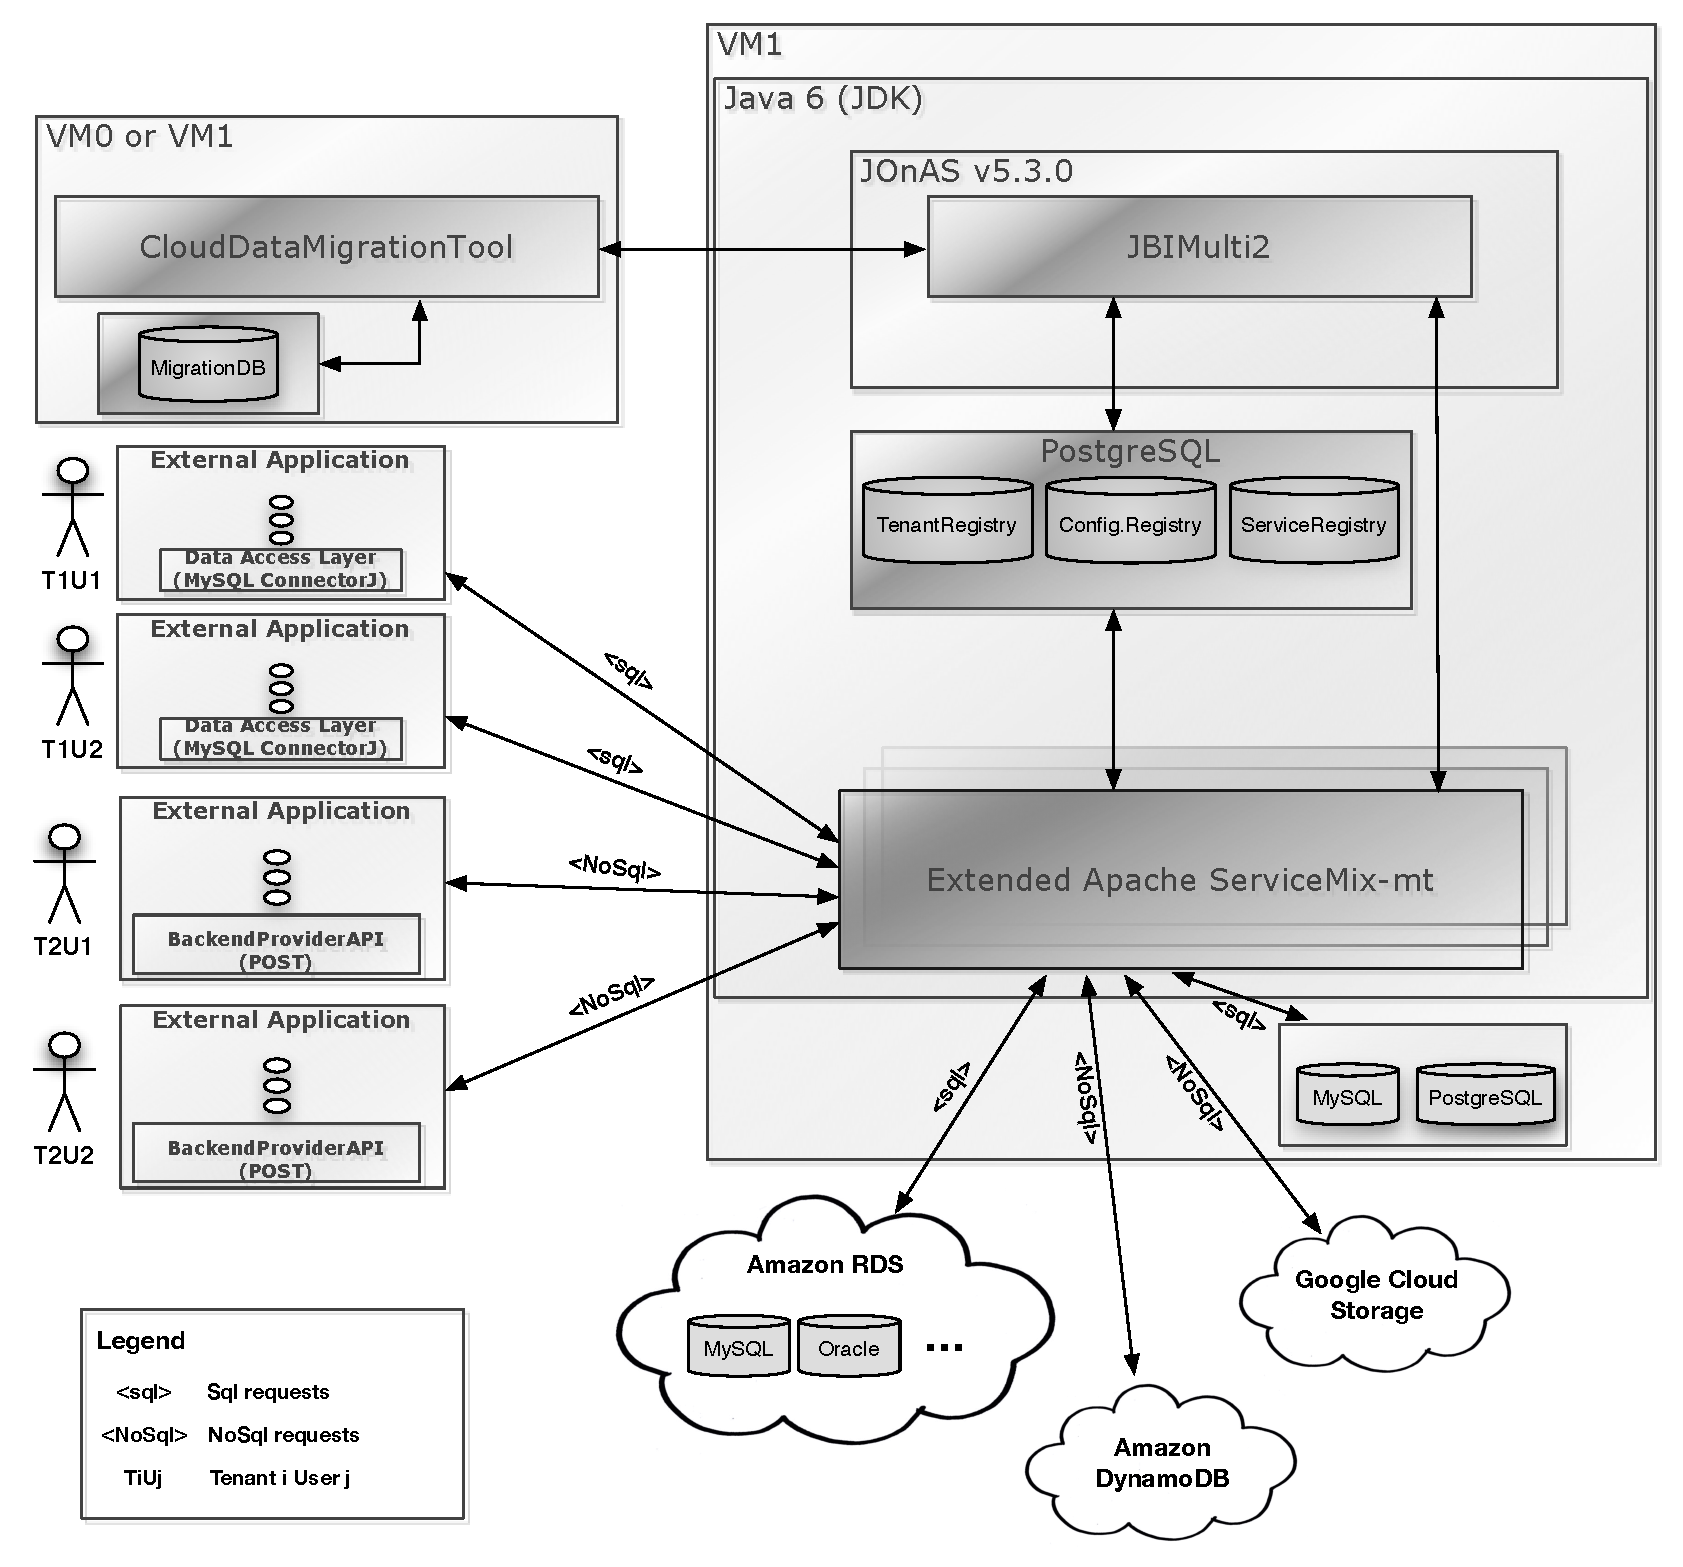
\includegraphics[clip, scale=0.5]{./gfx/systemoverview.pdf}
	\caption[Transparent Cloud Data Access System Overview]{Transparent Cloud data access system overview, including the \term{Cloud Data Migration Application} \cite{bachmann2012}. Note: represents the system in the post-migration phase}
	\label{fig:systemoverview}
\end{figure}

The transparent Cloud data access access support is achieved by the interaction of three main components: JBIMulti2, registries containing tenant-aware information, and an extended version of ServiceMix-mt (see Figure \ref{fig:systemoverview}). JBIMulti2 deploys in ServiceMix-mt the \ac{SA}s containing the endpoint and routing configurations selected by the tenant, which support two different communication protocols: MySQL and \ac{HTTP}. From this point the DAL of the tenant's application can retrieve and modify data in his data container in the Cloud through the \ac{ESB} connecting to a single logical endpoint which connects to multiple physical backend data stores. In our approach we provide also the possibility, either to configure a connection to the traditional database, e.g. when a hybrid model is pursued, or to utilize a \ac{DBMS} provided in our system, which is described in the following subsection.

%The JBIMulti2 utilizes three main components in the system: registries created in a PostgreSQL database, resources in ActiveMQ and ServiceMix. When deploying a tenant's \ac{SA} the application initiates an unidirectional communication to a management queue from which a management \ac{OSGi} bundle consumes the management messages from JBIMulti2 and performs managements operations in ServiceMix, such as deploy and undeploy. The deployed multi-tenant \ac{SA}s configure the tenants' endpoints for \ac{BC}s or \ac{SE}s. When deployed a multi-tenant \ac{SA} which packages a \ac{JMS} endpoint configuration, resources are transparently created in the out-of-the-box ActiveMQ instance which is shipped with ServiceMix. However, it is out of the scope of this student thesis an interface for connecting the different tenants with the created \ac{JMS} resources.


\FloatBarrier
\newpage
\chapter{Components}

%This chapter lists \ac{XSD}s that WS-Policy Assertion language and Rules XML file must conform. Furthermore, there are given several policy documents of Cloud data stores that are used for validation.

\section{CDASMix MySQL Proxy}
\label{appendix:cdasmixmysqlproxy}

The MySQL proxy \ac{OSGi} bundle is implemented on the Continuent Tungsten Connector \cite{tungstenwiki}, which is a Java MySQL proxy which directly connects with the backend MySQL database system. We extend and adapt this proxy in order to integrate it with ServiceMix, aggregate transparency, multi-tenant awareness, cashing, and dynamic connection with the backend Cloud data sources.

\begin{figure}[htb]
	\centering
		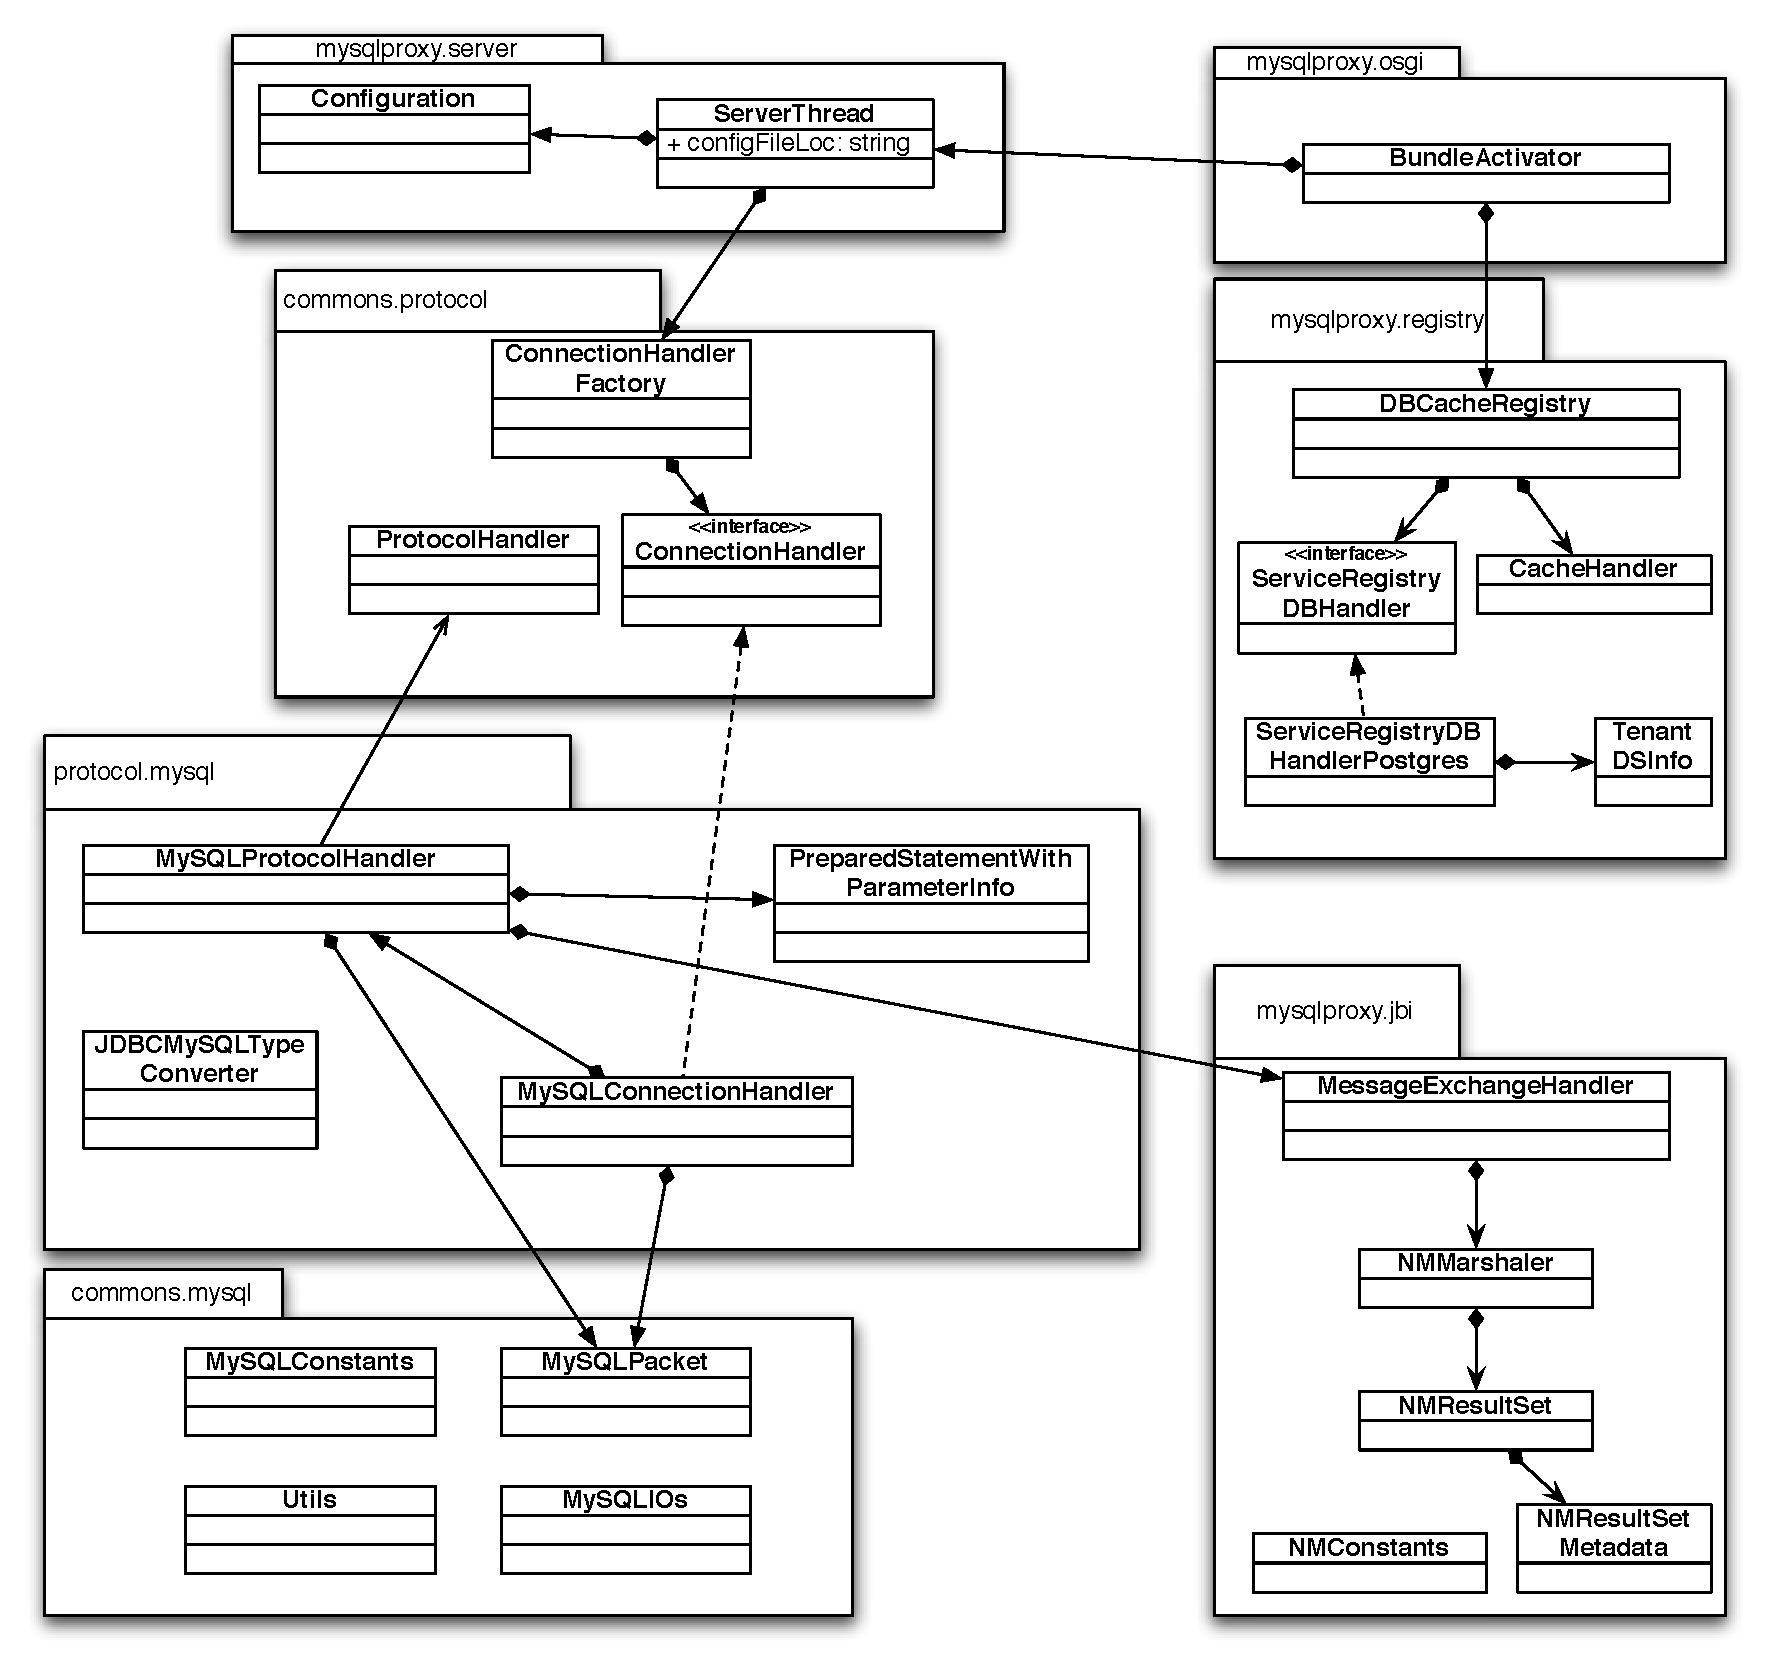
\includegraphics[clip, scale=0.4]{./gfx/mysql-osgi/mysql-proxy-v3.pdf}
	\caption[ServiceMix-mt MySQL OSGi Bundle]{OSGi bundle providing MySQL support in ServiceMix-mt}
	\label{fig:mysqlclassdiagram}
\end{figure}

\FloatBarrier

\vspace*{0.5cm}

%\lstinputlisting[label={lst:policy_language_syntax},caption={[Syntax of WS-Policy Assertion Language Schema]Syntax of WS-Policy Assertion Language Schema.},style=xml]{./gfx/master_thesis/cdhs-ws.xml}

%\vspace*{1cm}

%\vspace*{0.5cm}

%\lstinputlisting[label={lst:policy_language_schema},caption={[CDHS WS-Policy Assertion Language Schema]CDHS WS-Policy Assertion Language Schema.},style=xml]{./gfx/master_thesis/cdhs_properties.xsd}

%\vspace*{1cm}

\section{CDASMix Camel JDBC}
\label{subsec:cdasmixcameljdbc}

The \term{cdasmixjdbc} component is a custom component which is built and deployed as an \ac{OSGi} bundle in ServiceMix-mt. It provides support for connections with backend \ac{SQL} Cloud data stores, and message marshaling and demarshaling.

\begin{sidewaysfigure}[htb]
	\centering
		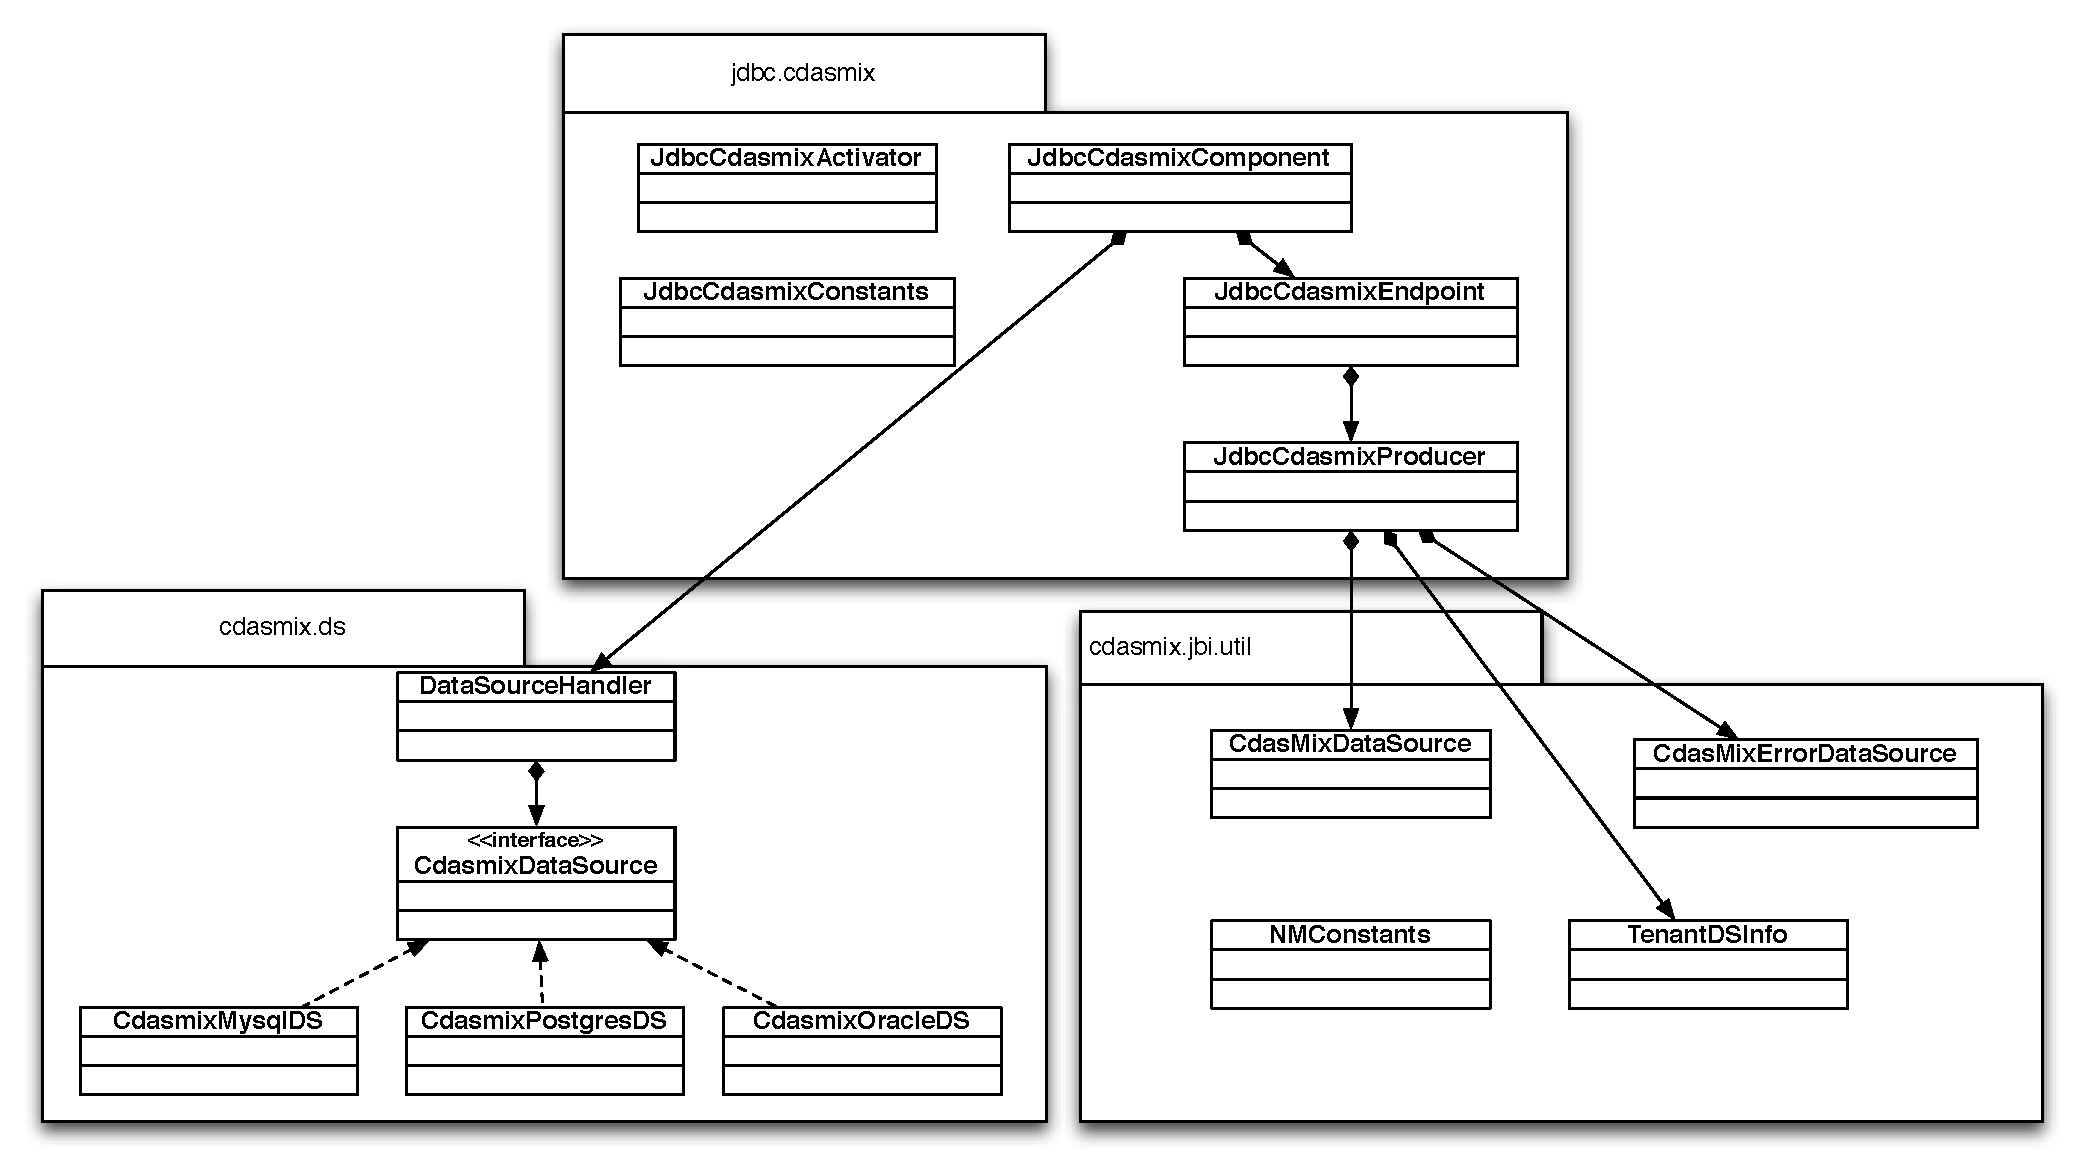
\includegraphics[clip, scale=0.6]{./gfx/cdasmix-camel-jdbc/cdasmix-camel-jdbc.pdf}
	\caption[ServiceMix-mt Camel CDASMix-JDBC Component]{OSGi bundle and Camel component providing JDBC support in ServiceMix-mt}
	\label{fig:cdasmixjdbcclassdiagram}
\end{sidewaysfigure}

\vspace*{0.5cm}

\FloatBarrier

%\lstinputlisting[label={lst:rules_schema},caption={[Post-Processing Rules XML Schema]Post-Processing Rules XML Schema.},style=xml]{./gfx/master_thesis/rules.xsd}

%\vspace*{1cm}

%\section{Multi-tenant ServiceMix HTTP Binding Component}
%\label{appendix:httpmtbc}

%to be filled
%\vspace*{0.5cm}

%\lstinputlisting[label={lst:googleCloudSQL-policy},caption={[Google Cloud SQL Service Provider Policy]Google Cloud SQL Service Provider Policy.},style=xml]{./gfx/master_thesis/provider_policies/GoogleCloudSQL.wspolicy}

%\vspace*{1cm}

%\vspace*{0.5cm}

%\lstinputlisting[label={lst:sqlDatabase-policy},caption={[SQL Database Service Provider Policy]SQL Database Service Provider Policy.},style=xml]{./gfx/master_thesis/provider_policies/SQLDatabase.wspolicy}

%\vspace*{1cm}
\FloatBarrier


\clearpage
\section{Multi-tenancy}
\label{sec:specificationmultitenancy}

In this section we detail the multi-tenant requirements the system must fulfill in order to ensure tenant-isolation at two levels: communication and storage. The final prototype must ensure a multi-tenant aware transparent access to data hosted in the Cloud. Although we provide storage support in our system for hosting migrated tenant's data (see Section \ref{sec:systemoverview}), it does not implement a multi-tenant storage model, because this is not a goal in our design. Therefore, we rely on the multi-tenant storage models different Cloud providers implement.

\subsection{Communication Requirements}

The final prototype must not only support a multi-tenant, but also a multi-protocol communication between endpoints. ServiceMix-mt is shipped with the following multi-tenant aware \ac{BC}s: \ac{HTTP}, \ac{JMS}, and E-mail \cite{gomez2012}. However, the existing communication protocols for data transfer purposes leads us to discard the \ac{JMS} and E-mail. \ac{RDBMS}, e.g. MySQL and PostgreSQL, implement their own protocol in their client/server model, at the \ac{TCP} level of the network stack. At the client side the protocol is supported by the native drivers provided to the developers, e.g. MySQL Connector/J, and at the server side by the different components which build the database server \cite{mysqlmanual}. This fact forces us to provide a vendor-oriented communication protocol environment, by providing support for the different protocols in independent components, rather than in a single standardized component.

Communication in, and from the \ac{ESB} must be multi-tenant aware. We divide the required isolation between tenants into the following sub-requirements: 

	\begin{itemize}
		\item \textbf{Tenant-aware messaging}: messages received in the \ac{ESB} and routed between the tenant-aware endpoints should be enriched with tenant and user information. 
		\item \textbf{Tenant-aware endpoints}: in ServiceMix-mt tenants pack a common endpoint configuration packed in a \ac{SU}, which is then deployed as a \ac{SA} in ServiceMix-mt's \ac{JBI} container \cite{gomez2012}. The multi-tenant aware \ac{BC} dynamically modify the endpoint's URL by injecting tenant context in it. In a database system in our scenario we do not have only tenants as the main actors, but also the different users which can access a tenant's database. Therefore, the tenant-aware endpoints should be dynamically created by injecting tenant and user information in the endpoint's URL. Furthermore, we must ensure tenant and user authentication in the system. 
		\item \textbf{Tenant-aware routing and context}: the deployment of tenant-aware endpoints should be followed by the creation of a tenant-aware context. Resources involved in a routing operation from one consumer endpoint to one provider endpoint can be shared between different tenants, but they must manage the routing operations in different tenant-aware contexts. The routing operations between two endpoints must identity the tenant and user who initiated the routing. 
		\item \textbf{Tenant configuration isolation}: configuration data persisted in our system should be isolated between tenants. A tenant's endpoint configuration data contains sensible information which identifies and allows access to the tenant's backend data stores. 
		\item \textbf{Tenant-aware correlation}: in a request-response operations, the response obtained from the backend data store must be correlated with the tenant's request to the system, and ensure that one tenant does not receive responses from another tenant's request.
	\end{itemize}

\subsection{Storage Requirements}

Due to the fact that our system does not primarily requires multi-tenant aware storage support, but we rely on multi-tenant aware storage systems in the Cloud, we summarize the main requirements for isolating data between tenants in database systems. 

Curino et al. identify as a primary requirement for a Cloud provider offering a \ac{DBaaS} model security and privacy \cite{relationalcloud2010}. A system running multiple database servers and each server multiple database instances must contain the necessary meta-data to provide tenant-aware routing in the system, and ensure that one tenant can only access the information in his database instance. Furthermore, privacy of stored data between tenants can be ensure by encrypting all tuples \cite{relationalcloud2}. Curino et al. introduce \term{CryptDB}, a subsystem of a relational Cloud which provide data encryption and unencryption functionalities for persisting data, and for accessing data via \ac{SQL} queries which are not aware of the encrypted storage mechanism in the system. However, it is known that the key challenge in managing encrypted data in the Cloud is doing it efficiently.

\FloatBarrier
\section{Dynamic Transparent Routing}
\label{sec:dynamicrouting}

Data access and modification from different back-end data stores must be supported in a transparent way between the tenants. We divide this requirement into two sub-requirements we consider our system must fulfill: Transparency, and Dynamic Routing.

\subsection{Transparency}

Giving a single logical view on a distributed database system abstracts the tenant from knowing the physical location of his data. The system must provide a single access endpoint for accessing and modifying data previously migrated to the Cloud. We must perform internally the necessary search operations in the registry containing the back-end data stores information, and the necessary mapping operations with the meta-data included in the tenants' requests. After those operations, our system must forward the requests to the back-end data stores and forward the responses to the tenants' requests.

\subsection{Dynamic Routing}
%dynamic between endpoitns and transformer
% dynamic between datasources, but no joins between different datasources
% dynamic between datasource with multi-querying option

Providing transparency by exposing a single endpoint to retrieve data from different back-end data stores requires the system to support dynamism in its routing mechanisms. One tenant may migrate one database to the Cloud, or \term{shard} a database between different databases in the Cloud, or different Cloud providers. This fact forces us to support connections to the back-end data stores dynamically rather than statically. Furthermore, when query and data transformation is required due to version or schema direct incompatibility between the tenant's requests and the back-end data store support, transformation mechanisms must ensure transformation of queries and data in order to provide a full transparent access. When transformations are not needed, the message should not be routed through a transformer component. In the prototype developed in this diploma thesis query and data transformations are out of scope.

When \term{sharding} a database, the tenant can split the data between two or more databases, or database systems. In order to minimize the changes in the application's DAL, we must support a single physical frontend endpoint while processing the tenant's request through one or more physical back-end endpoints. Special cases such as queries containing JOIN operations in between tables stored in different back-end \ac{SQL} databases are not supported. However, the system should support the execution of multiple \ac{SQL} queries in one request, which is known as \term{multiple-queries}.

\FloatBarrier
\section{Cache}
\label{sec:cache}

Cashing mechanisms in applications with high number of I/O operations benefits the application's performance, as described in Chapter \ref{chap:relatedworks}. The prototype developed in this diploma thesis provides support for application's I/O operations. Therefore, cashing is one of the main components which can drive to a better system performance. 

In our system the cache must be shared between the tenants using it. Hence, data cashed must be previously enriched with tenant and user context information. Operations in our system which require data from local or remote databases, e.g. authentication operations or data retrieval operations, should utilize the cashing mechanism to reduce the response time of the system. 

Tenant operations which perform changes in their data stored in the Cloud may lead to inconsistencies between the data persisted in the cache and the updated data in the Cloud. Freshness of data in the cashing system must be ensured.  

\FloatBarrier
\section{Integration Requirements}
\label{sec:intrequirements}

%integration with osgi and jbi, and look forward to the tendence of servicemix to eliminate the jbi compliance
%integrate it with the cloud migration tool
%integrate it with the future transformer of queries
%integrate the mysql protocol with the normalized message protocol

Apache ServiceMix 4.x versions are built on an \ac{OSGi}-based runtime kernel, Apache Karaf \cite{ASM}, \cite{Karaf2011}. However, they provide \ac{JBI} support for users migrating to newer versions. For new users it is recommended to consider \ac{JBI} deprecated, and build the components and expose the services in \ac{OSGi} \term{bundles}. We consider that developing our components as \ac{OSGi} \term{bundles} eases the compliance with newer versions in ServiceMix, and enables loose coupling between components. When a component is modified, the components in the \ac{OSGi} container which used the services of the modified component must not be redeployed. However, we find that the ServiceMix-mt component are \ac{JBI} compliant. We must then provide integration support between the \ac{JBI} components and the \ac{OSGi} \term{bundles}. The \ac{NMR} in ServiceMix eases the integration of the \ac{JBI} and \ac{OSGi} providing an \ac{API} for accessing the \ac{NMR} and creating message exchanges. However, the messages routed in ServiceMix-mt are in a \ac{NMF}, which is a completely different format with the message formats supported in the MySQL, or \ac{JSON} over \ac{HTTP} communication protocols. The system must ensure the appropriate conversion and mapping operations for marshaling and demarshaling incoming and outgoing messages. 

As described in previous sections, tenant's requests can be routed in ServiceMix-mt directly between one consumer and one provider tenant-aware endpoint when no query or data transformation is required. When transformation is required, we must design our components to be easily integrated with a future transformer component as an intermediary in the route between endpoints. 

JBIMulti2 is the application built on top on ServiceMix-mt to enable administration and managements operations on the \ac{ESB}. Therefore, the deployment of tenant-aware endpoint configurations can be only done through JBIMulti2. The \term{Cloud Data Migration Application} lacks of connection and access to the registries where the tenants' configuration data is stored. In order to avoid a database connection from the migration application, which may be hosted in an external server, to the registries which contain the tenant meta-data, we must provide an interface to allow either the tenant or the migration application to register the data store meta-data.

\newcommand{\usecase}[8]
{
{
\small \begin{longtable}{@{}p{.2\textwidth}p{.01\textwidth}p{.79\textwidth}@{}}
\toprule Name & & \textbf{#1} \\
\midrule Goal & & #2 \\
\midrule Actor & & #3 \\
\midrule Pre-Condition & & #4 \\
\midrule Post-Condition & & #5 \\
\midrule Post-Condition in Special Case & & #6 \\
\midrule Normal Case & \multicolumn{2}{p{.8\textwidth}}{\vspace*{-0.5cm}#7} \\
\midrule Special Cases &  \multicolumn{2}{p{.8\textwidth}}{\vspace*{-0.5cm}#8} \\
\bottomrule
\caption[Description of Use Case: #1]{Description of Use Case \term{#1}.}
\end{longtable}
}
\label{table:#1}
\clearpage
}


\section{Use Cases}
\label{sec:usecases}

In this section we extend the tenant operator use cases which are described in Muhler's and Uralov's approach \cite{Muhler2012}, \cite{Uralov2012}. The tenant operators are the users with less permissions in JBIMulti2, who perform service registration and endpoint configuration operations in ServiceMix-mt. An overview of the set of use cases for the tenant operators is presented in Figure \ref{fig:usecases}. The set of use cases we add to the previous version are highlighted, and described in detail. 

\begin{figure}[htb]
	\centering
		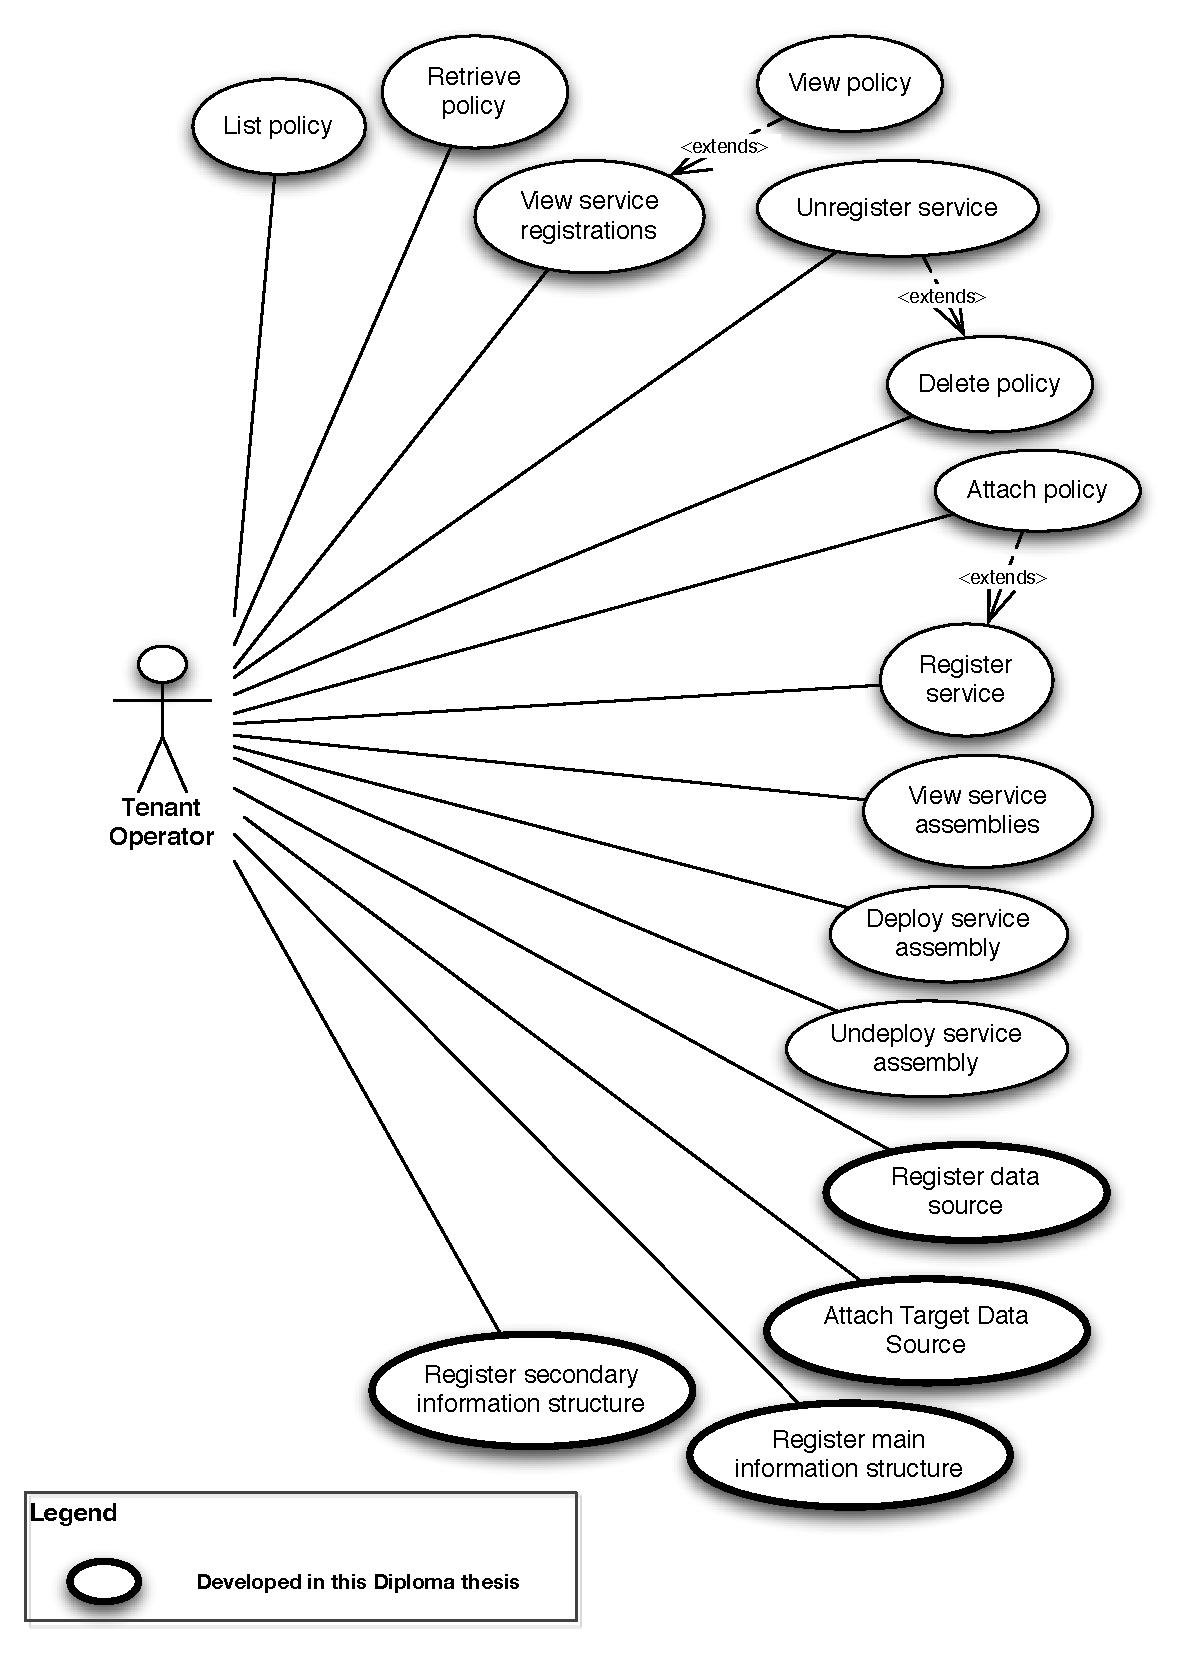
\includegraphics[clip, scale=0.59]{./gfx/usecaseDataSource.pdf}
	\caption[Use Case Diagram for Tenant Operator]{Use case diagram for tenant operator.}
	\label{fig:usecases}
\end{figure}

\pagebreak
\usecase{Register Data Source}
{The tenant operator wants to register a source and backend data source configuration data and associate it to an existing service assembly.}
{Tenant Operator}
{The tenant operator has the permissions in the service unit contingent and has registered a service assembly with no datasources associated to it.}
{Source and backend data source configuration data is stored successfully, and associated with a tenant's operator service assembly.}
{Source and backend data source configuration data are not stored, and not associated with the specified service assembly.}
{\begin{enumerate}
	\item The tenant operator selects the service assembly to which the data sources are associated.
	\item The source and target data sources configuration data are registered in the system, and associated to the specified service assembly.
\end{enumerate}}
{\begin{enumerate}
	\item[1a.] The service assembly does not exist.
		\begin{enumerate}
			\item The system shows an error message and aborts.
		\end{enumerate}
	\item[2a.] The service assembly is already associated with a source data source.
		\begin{enumerate}
			\item The system shows an error message and aborts.
		\end{enumerate}
	\item[2b.] The source data source configuration data already exists.
		\begin{enumerate}
			\item The system shows an error message and aborts.
		\end{enumerate}
	\item[2c.] The target data source configuration data already exists.
		\begin{enumerate}
			\item The system shows an error message and aborts.
		\end{enumerate}
\end{enumerate}}

\usecase{Attach Target Data Source}
{The tenant operator wants to attach one backend data source configuration data and associate it to an existing service assembly and source data source.}
{Tenant Operator}
{The tenant operator has the permissions in the service unit contingent and has registered a source data source.}
{The target data source is attached successfully to the specified source data source, and associated with the specified service assembly.}
{Target data source configuration data is not attached, and not associated with the specified service assembly.}
{\begin{enumerate}
	\item The tenant operator selects the service assembly to which the source data source is associated.
	\item The tenant operator selects the source data source to which the target data source must be associated.
	\item The target data source configuration data is attached to the specified source data source, and associated to the specified service assembly.
\end{enumerate}}
{\begin{enumerate}
	\item[1a.] The service assembly does not exist.
		\begin{enumerate}
			\item The system shows an error message and aborts.
		\end{enumerate}
	\item[2a.] The source data source does not exist.
		\begin{enumerate}
			\item The system shows an error message and aborts.
		\end{enumerate}
	\item[3a.] The target data source already exists.
		\begin{enumerate}
			\item The system shows an error message and aborts.
		\end{enumerate}
\end{enumerate}}

\usecase{Register Main Information Structure}
{The tenant operator registeres a main information structure and associate it with the specified source and target data source.}
{Tenant Operator}
{The tenant operator has the permissions in the service unit contingent and has registered the specified source and target data source.}
{The source and target main information structure meta-data is registered successfully, and associated with the specified source and target data source.}
{Source and target main information structure are not registered, and are not associated with the specified source and target data source.}
{\begin{enumerate}
	\item The tenant operator selects the service assembly to which the source data source is associated.
	\item The tenant operator selects the source and target data source to which the source and target main information structure is associated.
	\item The source and target main information structure are registered and associated with their source and target data source.
\end{enumerate}}
{\begin{enumerate}
	\item[1a.] The service assembly does not exist.
		\begin{enumerate}
			\item The system shows an error message and aborts.
		\end{enumerate}
	\item[2a.] The source or target data source does not exist.
		\begin{enumerate}
			\item The system shows an error message and aborts.
		\end{enumerate}
	\item[3a.] The main source or target information structure already exists.
		\begin{enumerate}
			\item The system shows an error message and aborts.
		\end{enumerate}
\end{enumerate}}

\usecase{Register Secondary Information Structure}
{The tenant operator registeres a secondary information structure and associates it with the specified source and target main information structure.}
{Tenant Operator}
{The tenant operator has the permissions in the service unit contingent, has registered a source and target data source, has registered a source and target main information structure, and the source and target datasources are \ac{NoSQL} databases.}
{The source and target secondary information structure meta-data are registered successfully, and associated with the specified source and target main information structure.}
{Source and target secondary information structure are not registered, and are not associated with the specified source and target main information structure.}
{\begin{enumerate}
	\item The tenant operator selects the service assembly to which the source data source is already associated.
	\item The tenant operator selects the source and target data source to which the main information structure are associated.
	\item The tenant operator selects the source and target main information structure to which the secondary information structure is associated.
	\item The source and target secondary information structure are registered and associated with their source and target main information structure.
\end{enumerate}}
{\begin{enumerate}
	\item[1a.] The service assembly does not exist.
		\begin{enumerate}
			\item The system shows an error message and aborts.
		\end{enumerate}
	\item[2a.] The source or target data source does not exist.
		\begin{enumerate}
			\item The system shows an error message and aborts.
		\end{enumerate}
	\item[2b.] The source and target data source is a MySQL database.
		\begin{enumerate}
			\item The system shows an error message and aborts.
		\end{enumerate}
	\item[3a.] The main source or target information structure does not exist.
		\begin{enumerate}
			\item The system shows an error message and aborts.
		\end{enumerate}
	\item[4a.] The secondary source or target information structure already exists.
		\begin{enumerate}
			\item The system shows an error message and aborts.
		\end{enumerate}
\end{enumerate}}



\FloatBarrier
\section{Web Service Interface}
\label{sec:wsinterface}

The system must provide an interface with a set of operations to allow both the tenants and the \term{Cloud Data Migration Application} to interact with the system and configure the connections between the single physical consumer endpoint and the multiple provider endpoints. 

\FloatBarrier
\section{Non-functional Requirements}
\label{sec:nonfunctionalrequirements}

In this section we list and describe the non-functional requirements our system must fulfill. The non-functional requirements described in this thesis are independent from the ones satisfied by the Cloud data store providers, which are specified in the Service Level Agreement between the Cloud provider and the user. 

\subsection{Security}
Securing the tenant context information in our system is one of the main requirements we must fulfill. Tenant context in our system does not only contains tenant configuration data, but also contains the necessary meta-data from the backend data sources, which include the databases schemas and its access credentials. In order to ensure confidentiality and integrity of the data migrated to the Cloud, tenant configuration data must be visible only to the system, and not transferred to third parties through the Web or Web service interface.

\subsection{Backward Compatibility}
In this diploma thesis we must face to two architectural tendencies in ServiceMix-mt: \ac{OSGi}-based components and \ac{JBI}-based components. Backward compatibility with the multi-tenant \ac{JBI} components developed in \cite{gomez2012}, \cite{Muhler2012}, and \cite{Essl2011} must be ensured. At the same time we must build the new components following the \ac{OSGi} tendency.

Compatibility with non multi-tenant aware endpoint configurations must be ensured in the system. In ServiceMix-mt we extend existing components, e.g. ServiceMix-http-mt, ServiceMix-camel-mt, JDBCCdasmix, etc., and deploy them as custom components. By deploying the extended components as separate custom components, we avoid conflicts with the non multi-tenant aware components ServiceMix is shipped with, e.g. ServiceMix-http \cite{ASM}, ServiceMix-camel \cite{ASM}, Camel-jdbc \cite{cameljdbc}, etc. Configuration of non multi-tenant aware endpoints is still supported in ServiceMix-mt. 

\subsection{Performance}
As discussed in previous sections, different performance indexes usually drive down in a system which relies on a high I/O operations number. Therefore, we must integrate additional mechanisms, e.g. cashing, in order to alleviate the performance fall. We mention in Chapter \ref{chap:relatedworks} not only performance benefits in terms of system efficiency when cashing, but also an economic efficiency when access to data involves an economic cost.

\subsection{Scalability and Extensibility}
The system should offer clustering functionality and scale appropriately in a Cloud infrastructure. JBIMulti2 enables administration and management of more than one instance of ServiceMix \cite{Muhler2012}. The horizontal scalability is out of the scope of this diploma thesis. This feature is contained in the diploma thesis "Extending an Open Source Enterprise Service Bus for Horizontal Scalability Support" \cite{Fest2012}. The integrated prototype should be upgradable and for this goal the decoupling of components have to facilitate changes in functionality. 

\subsection{Maintainability and Documentation}
The source code provided in this diploma thesis should be well commented and documented. The needed documentation should be shipped in the system's package in order to provide the necessary steps and tips to lead to a running system and possible future extensions. Furthermore, a test suite containing the main operations and data needed to run on the Web service interface to configure the system must be provided for future automation purposes. 



%In this section we identify the functional and non-functional requirements that the outcome of this thesis should comply to. The two approaches this thesis integrates identify several functional and non-functional requirements in administration and management, and communication in a multi-tenant aware \ac{ESB} solution \cite{Muhler2012}, \cite{Essl2011}. We fully adhere the former ones and we change, for performance and usability improvement, the latter ones. The outcome of this student thesis should be tested using the taxi scenario \cite{4CaaSt} described in Section \ref{sec:motivatingscenario}, and its performance should be evaluated using different scenarios based on the Direct Proxy Service scenario from the AndroitLogic \ac{ESB} Performance Round 6 \cite{androit2012}.  Both of the scenarios which are used in this thesis require two different integration requirements, which are described in the Sections \ref{subsec:intrequirements} and \ref{sec:evalrequirements}. 


%\subsubsection{Non-functional requirements}

%The extension of ServiceMix for multi-tenancy awareness we implement in this student thesis should conform to the following non-functional requirements:

%	\begin{itemize}
%		\item \textbf{Security:} the extended multi-tenant aware \ac{BC}s should implement security mechanisms. The tenant context information should be only visible to the tenant and the system, to avoid possible system attacks. The multi-tenant aware \ac{BC} should be capable of unencrypting the tenants' incoming messages and encrypting the routed outgoing messages from the system to the backend service. Encryption and unencryption are out of the scope of this student thesis. However, we provide each tenant consumer endpoint with a tenant authentication mechanism before creating the \ac{NM} and the message exchange. 
%		\item \textbf{Backward Compatibility:} Servicemix is shipped with non multi-tenant aware binding components. Therefore, we need our extended prototype to provide backward compatibility with the original \ac{BC} configurations and non multi-tenant aware communications.
%		\item \textbf{Performance:} the negative impact ServiceMix's performance due to the extension for enabling multi-tenancy awareness in the system should be minimized. Essl proposes the use of tenant context information which requires the retrieval of extra tenant information from a Tenant Registry before creating the message exchange \cite{Essl2011}. This implies an independent retrieval of data per request received in each tenant's consumer endpoint. The system should minimize the retrieval of external data to ServiceMix in order to minimize the performance penalty due to implementation of the multi-tenant communication approach.
%		\item \textbf{Scalability and Extensibility:} the integrated prototype should offer clustering functionality and scale appropriately in a Cloud infrastructure. JBIMulti2 complies administration and management between more than one instance of ServiceMix \cite{Muhler2012}. However, the communication to the system composed of two or more instances of ServiceMix should be managed in order to route the messages to a tenant's consumer endpoint located in one specific (or replicated in more than one) instance of ServiceMix. The Horizontal Scalability is out of the scope of this student thesis. This feature is contained in the diploma thesis "Extending an Open Source Enterprise Service Bus for Horizontal Scalability Support" \cite{Fest2012}. The integrated prototype should be upgradable and for this goal the decoupling of components have to facilitate changes in functionality. 
%		\item \textbf{Dynamic Service Discovery:} a multi-tenant aware \ac{ESB} in a Cloud environment must provide dynamic discovery of the services the tenants provide. For this purpose, the service broker can search the services which best fits for the consumer policy requirements. This functionality is out of the scope of this student thesis, but being implemented in the master thesis "Extending an Open Source Enterprise Service Bus for Dynamic Discovery and Selection of Cloud Data Hosting Solutions based on WS-Policy" \cite{Uralov2012}.
%		\item \textbf{Maintainability and Documentation:} the source code provided in this student thesis should be well commented and documented. Moreover, the provided documentation should be user friendly and should lead to a ease setting up and extending the system in the future. 
%	\end{itemize}




% integrate it with the orchestra container which speaks only soap, as well as with the different components
% synchronous communication with a variable timeout from the processes
% multi-tenant and non-multi tenant communication. The processes are not multi-tenant and the communication from the taxi company is multi-tenant, idem for the taxi transmitter
%The outcome of this student thesis must be integrated with the taxi scenario originated from the 4CaaSt project to build the taxi application \cite{4CaaSt}. For this purpose, and after analyzing the different components forming the taxi application, we need to specify additional requirements the system should fulfill for integration purposes. In the version two of the taxi application the point-to-point connections between the \ac{BPEL} processes installed in OW2 Orchestra and the Web services these consume have to be replaced with a communication through ServiceMix endpoints (Section \ref{sec:systemoverview}). The \ac{BPEL} processes installed in Orchestra communicate using \ac{SOAP} over \ac{HTTP} protocol. Furthermore, some of the components of the taxi application have to be multi-tenant aware to communicate with the tenant aware \ac{JBI} endpoints of the \ac{ESB} (e.g. TaxiCompany and TaxiTransmitter), and some components are non multi-tenant aware and have to communicate through non multi-tenant aware \ac{JBI} endpoints in ServiceMix (e.g. Processes installed in Orchestra, CMF and GoogleServices). As last requirement to fulfill, the taxi request is mainly Orchestrated by several \ac{BPEL} processes which communicate with different services to retrieve information and book a taxi. The overall process time is variable but synchronous. The multi-tenant endpoints correlating one tenant's taxi booking response have to be synchronized with the process replying the taxi request.






